% Auto-generated by generate_report.py — do not edit manually
% Preamble mirrors oxengthesis.cls so figures match the body text:
% Carlito as main font, Latin Modern Math via unicode-math.
\documentclass[border=6pt]{standalone}
\usepackage{fontspec}
\setmainfont{Carlito}
\usepackage{unicode-math}
\setmathfont{Latin Modern Math}
\usepackage{pgfplots}
\pgfplotsset{compat=1.18}
\usepgfplotslibrary{groupplots}
\usetikzlibrary{patterns,positioning}
\begin{document}
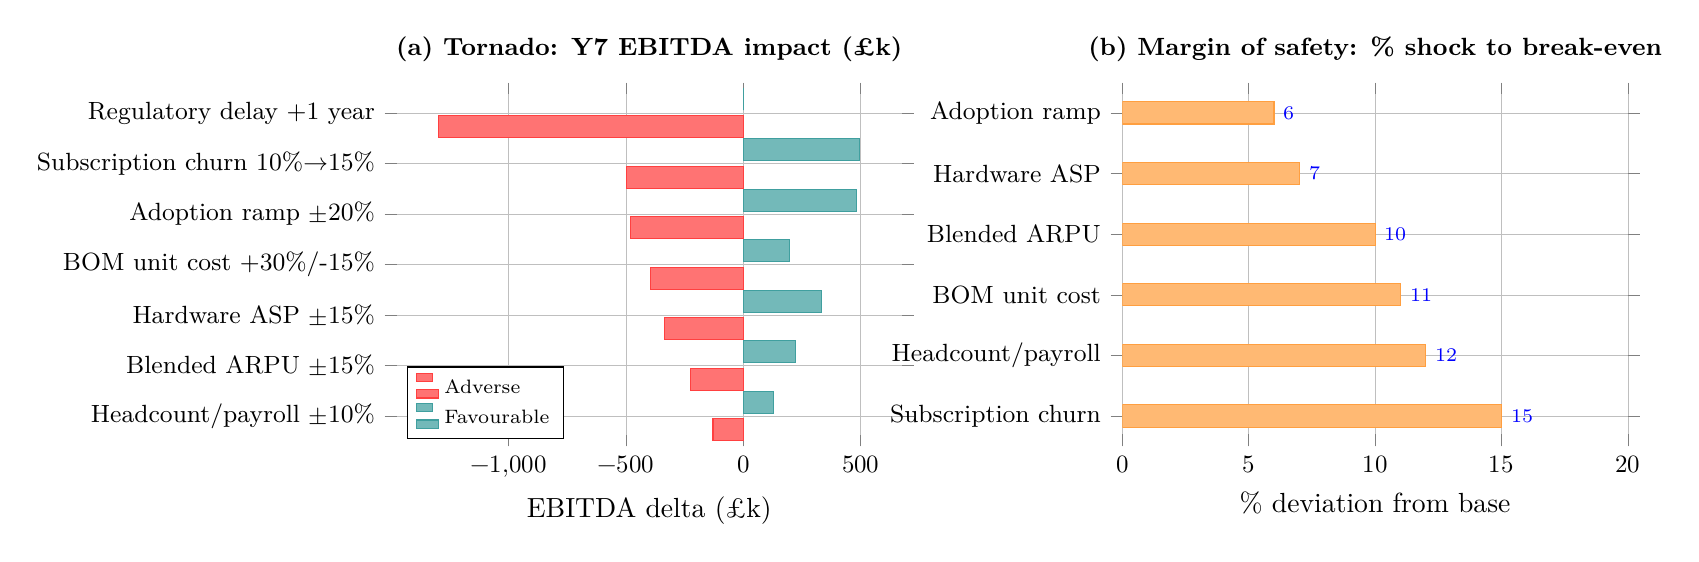
\begin{tikzpicture}
    \begin{groupplot}[
        group style={
            group size=2 by 1,
            horizontal sep=2.8cm,
        },
        width=8cm,
        height=6.2cm,
        tick label style={font=\small},
        label style={font=\normalsize},
        title style={font=\small\bfseries, yshift=-2pt},
        grid=major,
        grid style={line width=.1pt, draw=gray!30},
        major grid style={line width=.2pt, draw=gray!50},
    ]

    % --- Panel (a): Refined tornado ---
    \nextgroupplot[
        title={(a) Tornado: Y7 EBITDA impact (\pounds k)},
        xbar,
        bar width=8pt,
        xlabel={EBITDA delta (\pounds k)},
        symbolic y coords={{Headcount/payroll $\pm$10\%},{Blended ARPU $\pm$15\%},{Hardware ASP $\pm$15\%},{BOM unit cost +30\%/-15\%},{Adoption ramp $\pm$20\%},{Subscription churn 10\%$\to$15\%},{Regulatory delay +1 year}},
        ytick=data,
        y axis line style={opacity=0},
        enlarge y limits=0.10,
        legend style={
            at={(0.02,0.02)},
            anchor=south west,
            font=\scriptsize,
            cells={anchor=west},
        },
    ]
    \addplot+[xbar,fill=red!55,draw=red!75] coordinates {(-129,{Headcount/payroll $\pm$10\%}) (-223,{Blended ARPU $\pm$15\%}) (-334,{Hardware ASP $\pm$15\%}) (-395,{BOM unit cost +30\%/-15\%}) (-480,{Adoption ramp $\pm$20\%}) (-496,{Subscription churn 10\%$\to$15\%}) (-1297,{Regulatory delay +1 year})};
    \addplot+[xbar,fill=teal!55,draw=teal!75] coordinates {(129,{Headcount/payroll $\pm$10\%}) (223,{Blended ARPU $\pm$15\%}) (334,{Hardware ASP $\pm$15\%}) (198,{BOM unit cost +30\%/-15\%}) (480,{Adoption ramp $\pm$20\%}) (496,{Subscription churn 10\%$\to$15\%}) (0,{Regulatory delay +1 year})};
    \legend{Adverse, Favourable}

    % --- Panel (b): Margin of safety ---
    \nextgroupplot[
        title={(b) Margin of safety: \% shock to break-even},
        xbar,
        bar width=8pt,
        xlabel={\% deviation from base},
        symbolic y coords={{Subscription churn},{Headcount/payroll},{BOM unit cost},{Blended ARPU},{Hardware ASP},{Adoption ramp}},
        ytick=data,
        y axis line style={opacity=0},
        enlarge y limits=0.10,
        nodes near coords,
        nodes near coords style={font=\scriptsize},
        nodes near coords align={horizontal},
        xmin=0, xmax=20,
    ]
    \addplot+[xbar,fill=orange!55,draw=orange!75] coordinates {(15,{Subscription churn}) (12,{Headcount/payroll}) (11,{BOM unit cost}) (10,{Blended ARPU}) (7,{Hardware ASP}) (6,{Adoption ramp})};

    \end{groupplot}
\end{tikzpicture}

\end{document}
